\chapter{Evaluation}

SynVisio was made publicly available to use for free on the internet on September 2018. A stable version was deployed in the start of 2019 and ever since then, it has been used by several researchers across the world in exploring genomic conservation in a wide variety of organisms. To evaluate our system we conducted semi-structured interviews with 5 domain experts from the three research groups we were collaborating with and one of the expert was a bioinformatician who worked across all three research groups. The interviews were conducted either through phone or an in person meeting and lasted around 45-60 minutes. Researchers were first asked about the relevance of synteny visualizations in their field of research and then asked to give their opinion on the different features that SynVisio offers and how they helped in exploring synteny in their particular dataset. We summarize their feedback on the system through three case studies, one from each research collaborator group, presented in the sections below. To provide evidence on the effectiveness of our system \textit{in the wild} we explored user activity logs on the website for a period of 12 months through google analytics. Finally to demonstrate the open-ended design of SynVisio we provide an example of a genome database for silk worm that was extended to show synteny visualizations using the open sourced code of SynVisio.

\section{Case Studies}

\subsection{Wheat\textit{(Triticum aestivum)}}
What is one of the most widely cultivated crops in the world and plays an important role in human nutrition. Being a common cereal wheat genomes are highly diverse and spread over a large geographical range. The genome is capable of tolerating mutations and extensive hybridization to a great level which is why it has been able to adapt to such a wide variety of environmental conditions\cite{wheatinfo,10wheat}. Wheat is also one of the \textit{neolithic founder crops} that were the first to be domesticated almost 10000 years ago.
Bread wheat(AABBDD) is a hexaploid genome and is the result of series of hybridization events between three ancestral genomes A Donor(Triticum urartu), B Donor(Aegilops speltoides) and D Donor(Aegilops tauschii) which makes it an interesting subject for synteny analysis. Our collaborators were part of a research team involved in sequencing a high quality version of the wheat genome. Since the wheat genome is extremely large and complex synteny analysis can help researchers in assessing the quality and contiguity of the genome assembly though alignments between the sub genomes (A,B and D).

Our collaborators relied on visualizations generated by SynVisio to present and summarize their sequence assembly results - \textit{``the images have been used in presentations, academic meetings such as the international wheat congress and also at the plant-animal genome conference.'' (R1)}. While they used Circos style plots for research publications earlier, they mentioned that the multi level representations in SynVisio were far more useful for genomes like wheat with many chromosomes in it - \textit{``This tool is better than a Circos plot, especially when comparing multiple genomes, circos can be limited because you are seeing too many chromosomes in one circle and so are losing information ... a stacked layout like yours is easier to see.'' (R4)}. One collaborator in particular also appreciated the system for its ability to handle large datasets like wheat - \textit{``this is really neat. this is also very useful...a single wheat chromosome is vast and wheat has 21 of those placing stress on an analysis pipeline in terms of computational complexity...it is also very repetitive...'' (R1)}.
Feedback provided by this research team was also used in adding support for hive plots which offer a very intuitive representation to compare multi sub genomes in crops like wheat as shown in figure \ref{fig:ch_6_wheat}. The researchers in this team plan on publishing images generated using SynVisio and have already used it to create a portal for researchers to compare 12 different wheat cultivars for the 10+ Wheat Genomes Project. Users can use this portal to select any two varieties from 12 different wheat cultivars and then compare genomic conservation between them using SynVisio\cite{10wheat,wheatinfogithub}.

\begin{figure}
  \centering
  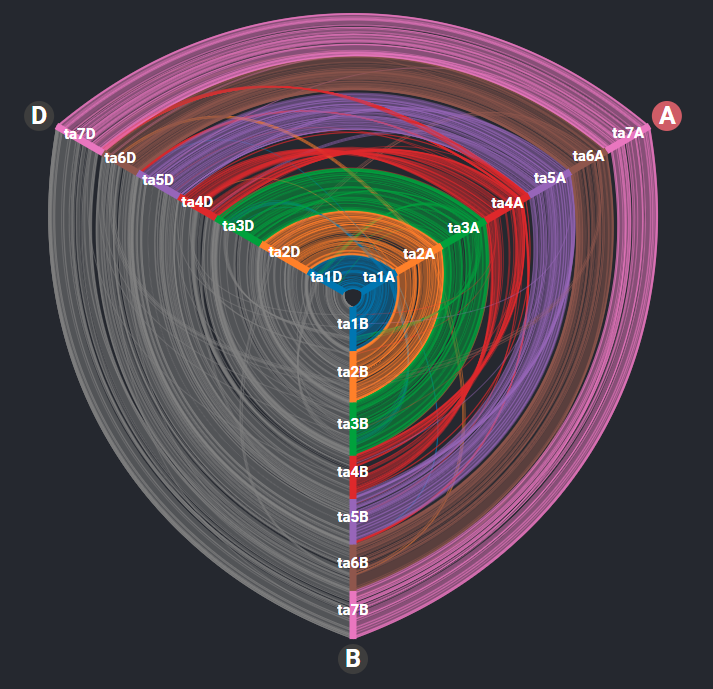
\includegraphics[width=0.72\linewidth]{images/ch_6_wheat.PNG}
  \captionof{figure}{Genomic conservation between the three sub genomes A,B and D of Wheat(Chinese Spring Variety) shown through a Hive plot in SynVisio.}
  \label{fig:ch_6_wheat}
\end{figure}


\begin{figure}
  \centering
  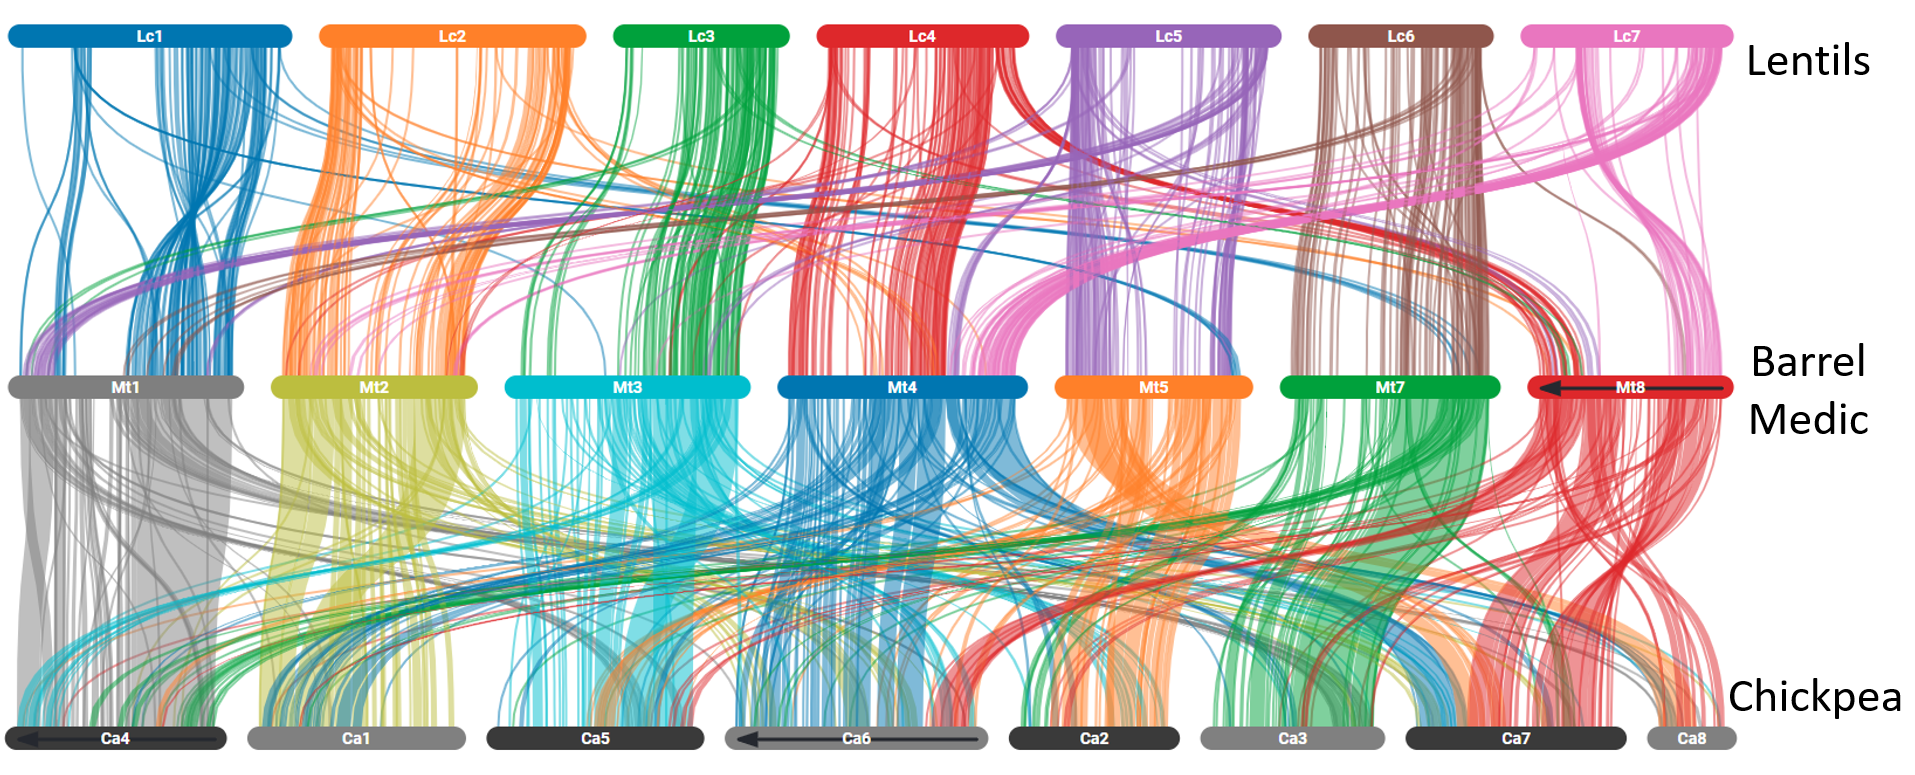
\includegraphics[width=1\linewidth]{images/ch_6_lentils.png}
  \captionof{figure}{Collinearity between Lentils(Lc), Barrel Medic(Mt) and Chickpea(Ca) presented through a Tree view plot. The ordering(Ca) and orientation(Mt8,Ca4 and Ca6 - flipped) of some chromosomes have been changed to reduce visual clutter.}
  \label{fig:ch_6_lentils}
\end{figure}


\subsection{Lentils\textit{(Lens culinaris)}}
Lentil is an important legume crop that is grown globally as a valuable source for dietary protein. It also plays a crucial role in food security in developing countries along with open legume crops like Chickpea(Cicer arietinum)\cite{varshney2013draft}. Lentils can be made more resistant to diseases and weed infestations by increasing the genetic diversity of the genome through hybridization between disease resistant wild varieties. This however requires mapping the traits through molecular markers to assess their diversity. Our collaborators relied on comparative genomic mapping to leverage information from a model legume species like Barrel Medic(Medicago truncatula) onto less studied crop species like lentils and chickpea due to lack of common markers.

Unlike the wheat genome, synteny analysis requirements for this project were centered around cross synteny between species rather than self synteny. Due to the large size difference in the genomes between Lentils(4Gbp) and Chickpea(~740Mbp) the first version of SynVisio was not able to generate legible charts as the Lentil chromosomes were extremely wide compared to chromosomes from the other species and so a special feature was added to have variable scales at different levels. Our collaborators were pleased with the updated view and also remarked on the multiple visual representations provided in the genome view - \textit{``I think it's quite good, I do really like that there's also the dot plot, in the corner, so that if anything is a little bit unclear, from the parallel view, you can kind of refer back to that.
'' (R5)}. Because this was a cross synteny analysis between several genomes, researchers mentioned that the Tree view was particularly helpful in summarising large scale chromosomal rearrangements and inversions while still keeping the different genomes visually distinct as shown in figure \ref{fig:ch_6_lentils}. They also compared it to circos plots and remarked on its usability - \textit{``It's like the circos plots are beautiful but you can't do anything with it. Whereas this, the tree-view in particular, is very aesthetically pleasing and that's the kind of thing that you can show to your collaborators and you can also understand it, at the same time, and then the interactive nature of it helps too...
(R5)''}. Reseachers froom this group have also used SynVisio to study genomic conservation in other legumes like the Tepary Bean (Phaseolus acutifolius) and are planing on using it to generate images for their research publications in future.

\subsection{Canola (Brassica napus)}




\section{Usage analysis based on Google Analytics Logs}


 
Methods – How we instrumented the program to gather the data.
Decide on a set of interview questions 
Come up with the interview format – Where they use the tool and then they describe the tool
Which views do they most often.
What are the advantages and we an ask them the question does this solve the problem of interactivity – WE ask them how they did it before and if this tool solves it ?
Compare no of steps used to create a chart before and after synvisio.

\section{Case Studies}
4 Case studies one for each person.

\section{Interpretations and Findings}  
Summarize what worked well and what didn’t work well .
Which sections where used frequently and why 
How are we doing on these initial problems – What we set to do and how has our system performed.
For example Availability – Just show the internet logs

